\section[Theorie]{{Theorie\footnote{Unter Verwendung der Quelle \cite{man:v601}.}}}

\subsection{Grundlagen}
\label{sec:grundlagen}
Der Franck-Hertz-Versuch ist ein Elektronenstoßexperiment. 
In diesem Zusammenhang bedeutet das, dass Hg-Atome mit Elektronen möglichst monoenergetischer Energie beschossen werden.
Es treten sowohl elastische als auch inelastische Stöße auf.
%Die kinetische Energie $E_\text{kin}$, die die Elektronen bei den inelastischen Stößen abgeben, dient dabei als Informationsquelle.
Bei einem inelastischen Stoß wird ein Hg-Atom aus seinem Grundzustand mit der Energie $E_0$ in den ersten angeregten Zustand mit der Energie $E_1$ versetzt.
Somit entspricht die Energiedifferenz 
\begin{align}
    E_{\text{kin,vor}} - E_{\text{kin,nach}} = \frac{m_0}{2} \left(v^2_\text{vor} -v^2_\text{nach}\right) = E_1 - E_0,
    \label{eq:energiedifferenz}
\end{align}
wobei $m_0$ die Ruhemasse und $E_\text{kin}$ die kinetische Energie des Elektrons ist.
Dabei sei angemerkt, dass theoretisch auch höhere Energieniveaus möglich sind, diese allerdings mit der hier verwendeten Apparatur nicht erreicht werden.
Ferner ist es nicht möglich, die Energie der emittierten Photonen beim Wechsel zurück in den Grundzustand zu messen.
Die Energiemessung der Elektronen erfolgt mittels der Gegenfeldmethode.



\subsection{Aufbau und Ablauf des Versuchs}
Der schematische Aufbau des Franck-Hertz-Versuchs ist in Abbildung \ref{fig:schematischer_aufbau} zu sehen.
\begin{figure}[H]
    \centering
    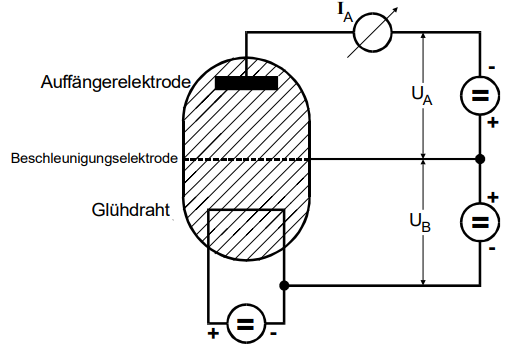
\includegraphics[height = 6.5cm]{bilder/schema.png}
    \caption{Schematischer Aufbau des Versuchs \cite{man:v601}.}
    \label{fig:schematischer_aufbau}
\end{figure}
\noindent
In dem evakuierten Glaskolben befindet sich ein kleiner Tropfen Quecksilber, welcher teilweise spontan verdampft bis sich gemäß der 
Dampfdruck-Kurve\footnote{vgl. \cite{man:v203}.} eine temperaturabhängige Sättigung $p_\text{sät}$ einstellt.
Folglich kann über die Temperatur $T$ die Dampfdichte des Quecksilbers gesteuert werden.
In dem Gefäß befindet sich ein Glühdraht aus einem hochschmelzendem Metall, z.B. Wolfram.
Dieser wird durch eine angeschlossene Gleichspannungsquelle bis auf Rotglut erhitzt, 
sodass gemäß des glühelektrischen Effektes Elektronen aus dem Draht gelöst werden.
Bei gegebener Temperatur wird dieser Effekt dadurch verstärkt, dass der Draht mit dem Oxid eines Erdalkalimetalls bestrichen wird,
welches eine niedrigere Austrittsarbeit als Wolfram hat.
Außerdem befindet sich eine netzförmige Beschleunigungselektrode im Gefäß, die von außen mit einer positiven Gleichspannung $U_\text{b}$
betrieben wird.
Durch das entstehende elektrische Feld werden die Elektronen zur Elektrode hin beschleunigt.
Falls die Elektronen vorher in Ruhe waren, gilt für sie nach der Beschleunigungsstrecke
\begin{align}
    \frac{1}{2} m_0 v^2_\text{vor} = e_0 U_\text{B}, 
    \label{eq:beschleunigung}
\end{align}
\noindent wobei $e_0$ die Elementarladung ist.

\noindent
Zum Messen des Auffängerstroms $I_\text{A}$ befindet sich eine Auffängerelektrode hinter der Beschleunigungselektrode,
die an eine Gegenspannungsquelle $U_\text{A}$ angeschlossen ist und ein Gegenfeld erzeugt.
Somit können nur solche Elektronen mit Geschwindigkeit $v_\text{z}$ in $z$-Richtung die Auffängerelektrode erreichen, die 
\begin{align}
    \frac{1}{2} m_0 v^2_\text{z} \geq e_0 U_\text{A}
\end{align}
erfüllen.

\noindent
Wie in Abschnitt \ref{sec:grundlagen} beschrieben finden sowohl elastische als auch inelastische Stöße zwischen Elektronen und Hg-Atomen statt.
Dabei gibt es je nach Elektronenenergie zwei Fälle.
Falls die kinetische Energie der Elektronen nicht ausreicht, kommt es ausschließlich zu elastischen Stößen.
Aufgrund des großen Massenunterschieds zwischen Elektron und Hg-Atom ist die abgegebene Energie des Elektrons vernachlässigbar gering,
obwohl es enorme Richtungsänderungen erfahren kann.
Falls $U_\text{B}$ so weit erhöht wird, 
dass die kinetische Energie der Elektronen mindestens der Energiedifferenz $E_1 - E_0$ aus Formel \eqref{eq:energiedifferenz} entspricht,
kann das Hg-Atom durch das Elektron in seinen ersten Angeregeten Zustand versetzt werden.
Nach einer Relaxationszeit der Größenordnung $\qty{10}{\nano\second}$ springt das Atom in seinen Grundzustand zurück.
Dabei wird ein Photon mit Frequenz $\nu$ der und der Energie 
\begin{align}
    E_1 - E_0 = h \nu
    \label{eq:photon}
\end{align}
emittiert, wobei $h$ das Plancksche Wirkungsquantum ist.

\noindent
Misst man $I_\text{A}$ in Abhängigkeit von $U_\text{B}$ bei konstantem $U_\text{A} < U_\text{B}$, 
so ergibt sich im Idealfall ein Plot wie in Abbildung \ref{fig:f-h-ideal}.
Anhand der vorhanden Peaks kann die Anregungsenergie bzw. ein ganzzahliges Vielfaches der Anregungsenergie abgelesen werden.
\begin{figure}[H]
    \centering
    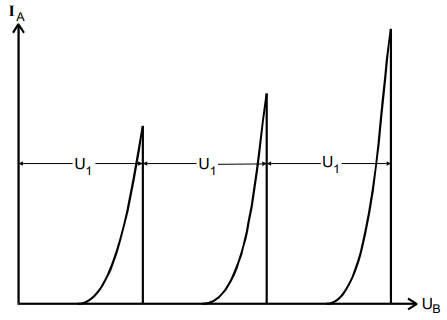
\includegraphics[height = 6.5cm]{bilder/franck-hertz-ideal.png}
    \caption{Ideale Franck-Hertz-Kurve \cite{man:v601}.}
    \label{fig:f-h-ideal}
\end{figure}
\noindent
